\chapter{Diseño de la interfaz de explicaciones}
\label{cap:interfaz}

El objetivo de nuestro proyecto, como ya hemos expresado anteriormente en este documento, consiste en proporcionar explicaciones que justifiquen la relación existente entre dos canciones proporcionadas por un recomendador de música. Una vez realizado el estudio de las canciones y las distintas explicaciones posibles, es necesario mostrar el resultado de nuestro estudio de una forma gráfica, comprensible para un usuario humano.\\

Los datos que manejamos en nuestro estudio consisten en objetos y las relaciones que existen entre ellos, pues siguen el modelo de datos RDF. Necesitamos representar todos los caminos que se forman entre las dos canciones iniciales, mostrando las conexiones existentes entre los objetos intermedios. Por estos motivos hemos decidido llevar a cabo la visualización mediante un grafo porque consideramos que se adecúa mejor a nuestras necesidades.\\

Es importante que la interfaz sea fácil de entender y usar, así que siempre trataremos de mantenerla lo más sencilla posible. La base de nuestro diseño es el grafo de explicaciones ya mencionado, pues es el elemento más importante debido a la gran cantidad de información que aporta y, por lo tanto, es también la parte central de la interfaz alrededor de la cual se posicionarán el resto de elementos.\\

\section{Diseño del grafo}

\begin{figure}[h!]
	\centering
	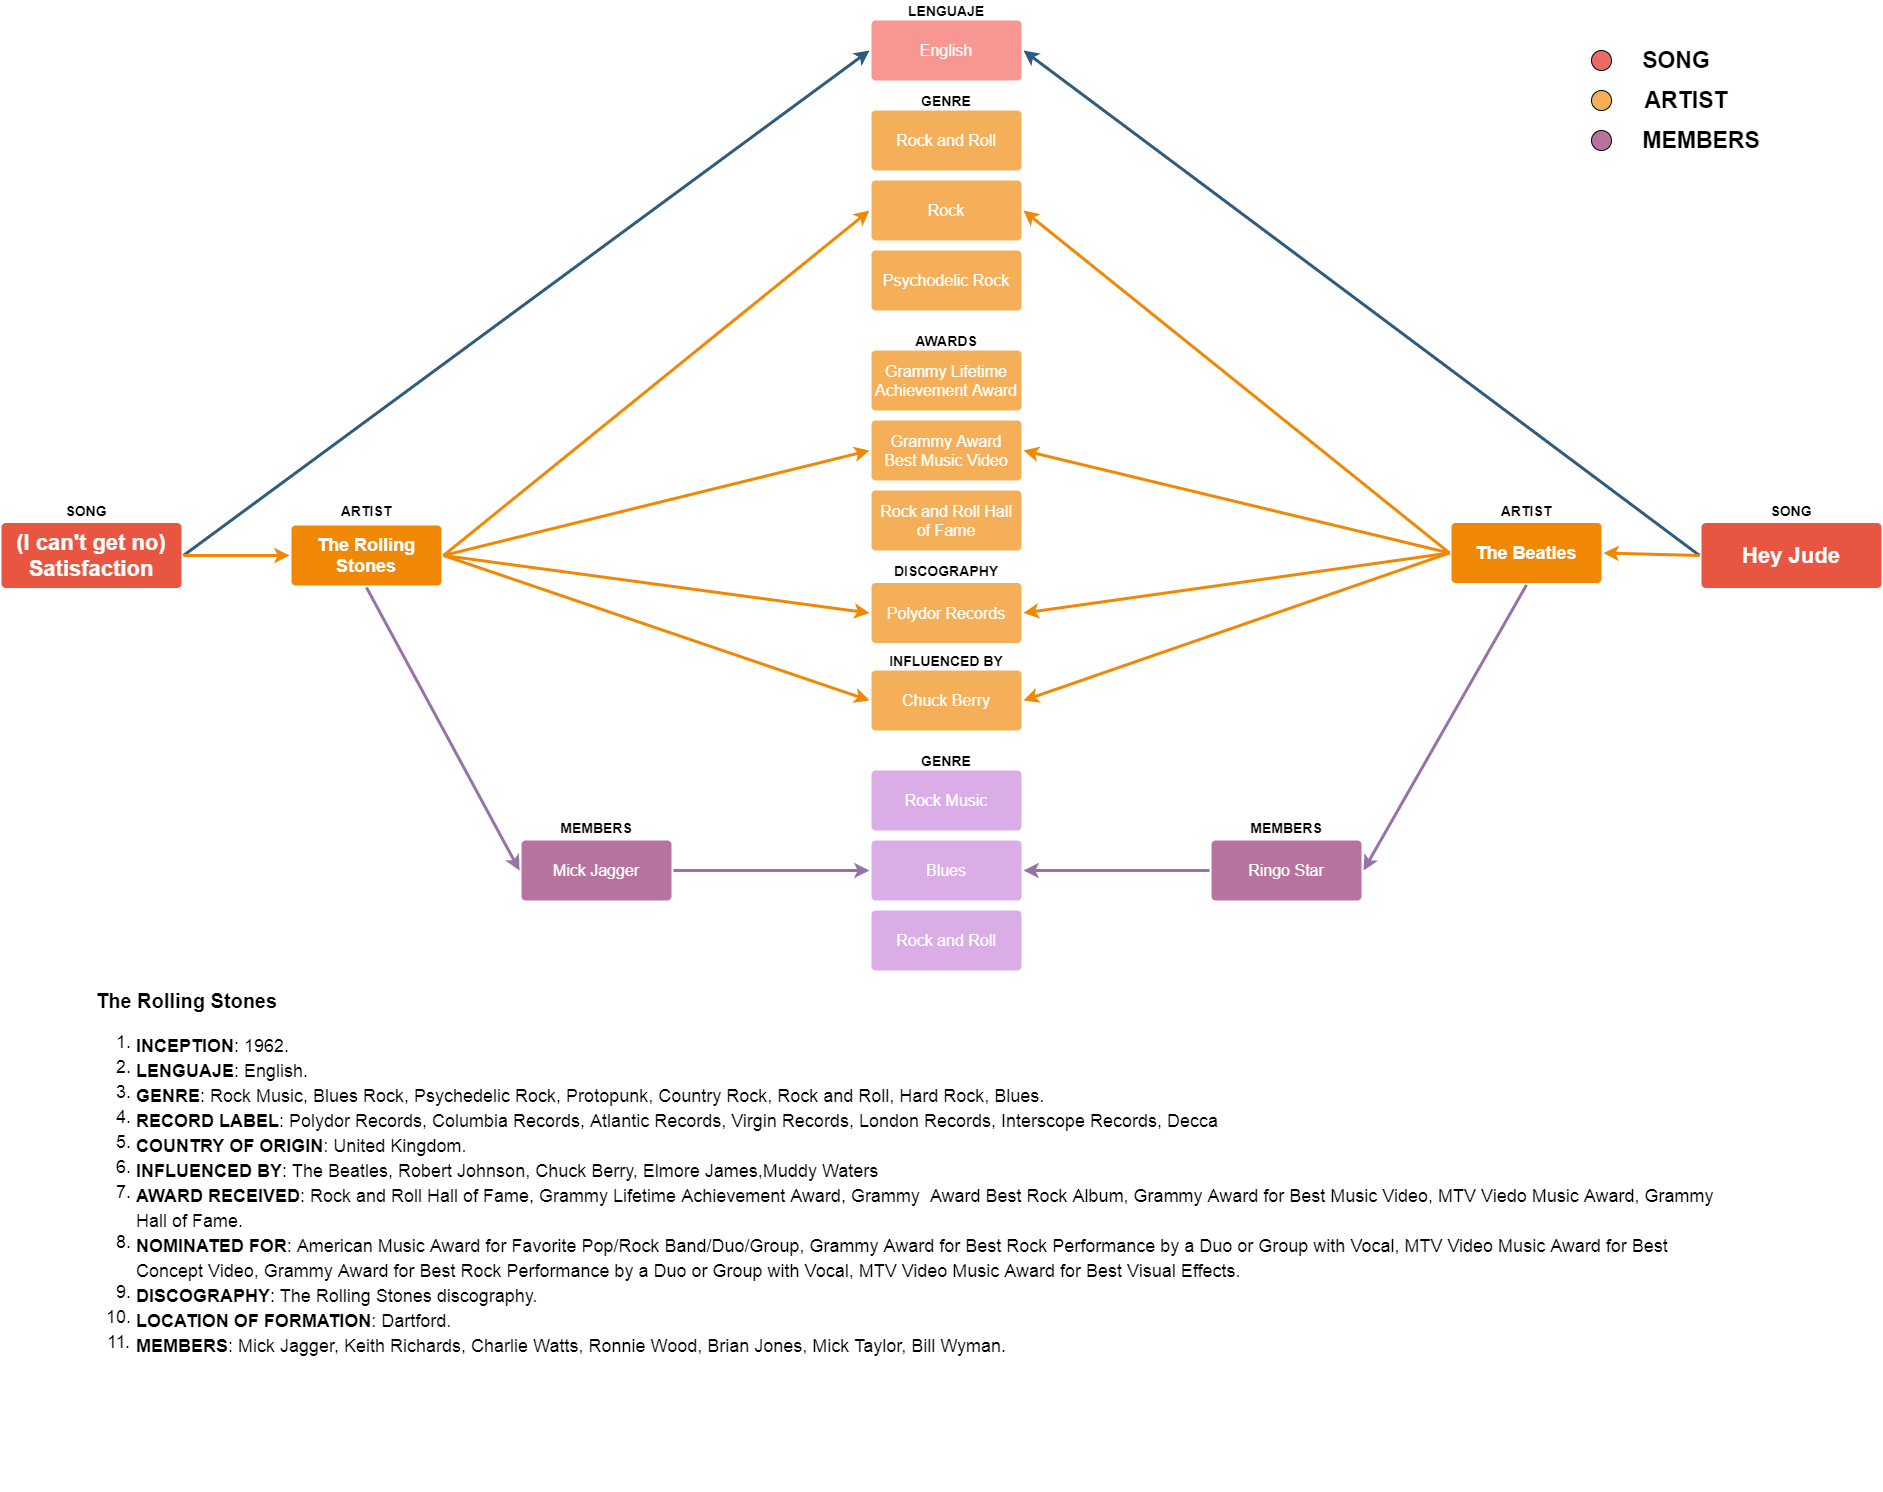
\includegraphics[width = 1\textwidth]{Imagenes/Bitmap/InterfaceResult.png}
	\caption{Primer diseño de la interfaz web}
	\label{fig:sampleImage}
\end{figure}

En la Figura 4.1 se puede observar la primera iteración de nuestro diseño. En ella se ve un ejemplo de grafo donde los nodos son los distintos sujetos y objetos (según el modelo RDF), mientras que las aristas representan los predicados que relacionan a esos nodos.\\

Los nodos están coloreados de manera diferente en función de su categoría. El color rojo está asociado a los nodos de las \textbf{canciones}, el naranja a los nodos de los \textbf{artistas} y el morado a los nodos de los \textbf{miembros} de esos artistas (en el caso de que estos artistas sean agrupaciones musicales). Los nodos centrales, correspondientes a los objetos de las explicaciones, tienen los mismos colores que los nodos de los que proceden pero con un tono más suave para diferenciarlos.\\

Los nodos rojos posicionados a ambos extremos son las canciones sobre las que estamos realizando el estudio. A partir de ellas parten todas las explicaciones. En el centro se puede ver también un nodo coloreado de un rojo más suave, este representa al objeto de una explicación directa (en este caso la explicación ``Idioma'').\\

Los nodos coloreados de color naranja representan los artistas de ambas canciones y las relaciones que existen entre ellos, de la misma forma que en el anterior caso con las canciones y las explicaciones directas. Estas explicaciones obtenidas por el estudio de los artistas son indirectas, ya que requieren un estudio más profundo para relacionar las canciones originales.\\

Por último, tenemos nodos morados que representan a los miembros o integrantes de los artistas, pues en este caso dichos artistas son bandas formadas por varias personas. Su funcionamiento es el mismo que el descrito en el párrafo anterior, con la salvedad de que estos miembros se obtienen del artista y, por lo tanto, sus explicaciones presentan un nivel extra de profundidad. Las explicaciones obtenidas de estos miembros son indirectas, ya que no proceden de las canciones en sí, y se representan con nodos de un morado más claro.\\

En esta versión del diseño también se propone una funcionalidad que permite visualizar datos adicionales. Haciendo click en los nodos sobre los que se hacen los estudios principales (canciones y artistas), se despliega una sección inferior en la que se muestran todos los datos obtenidos en el estudio del elemento concreto, aparezcan en el grafo o no. Así podemos ver todos los sellos discográficos con los que trabajaron \textbf{The Rolling Stones} aunque solo \textbf{Polydor Records} los relacione con \textbf{The Beatles}.\\

Esta función no es integral para el objetivo de nuestro proyecto, tan solo es un complemento que ofrece opciones al usuario, pero consideramos que puede ser un añadido interesante.\\

\section{Diseño básico de la interfaz}

Pasaremos ahora a explicar el resto de la interfaz con la ayuda de la Figura 4.2. En esta iteración, el diseño del grafo se mantiene intacto salvo un par de excepciones:

\begin{itemize}
\item Se han cambiado los colores que muestran las distintas categorías de los nodos. Ahora los nodos de las canciones y las explicaciones directas entre ellas son de color azul, los correspondientes a los artistas son de color rojo y los nodos de los miembros de los artistas son de color violeta. La decisión de cambiar estos colores se tomó para mejorar la visibilidad y obtener un grafo con mejor estética.\\

\item La segunda novedad, más relevante que la primera, es que se ha ampliado la lista de explicaciones indirectas mostradas en el grafo. Ahora se incluyen las explicaciones obtenidas del estudio de los géneros musicales de la canción y se representan con nodos de color verde.\\
\end{itemize}


\begin{figure}[h!]
	\centering
	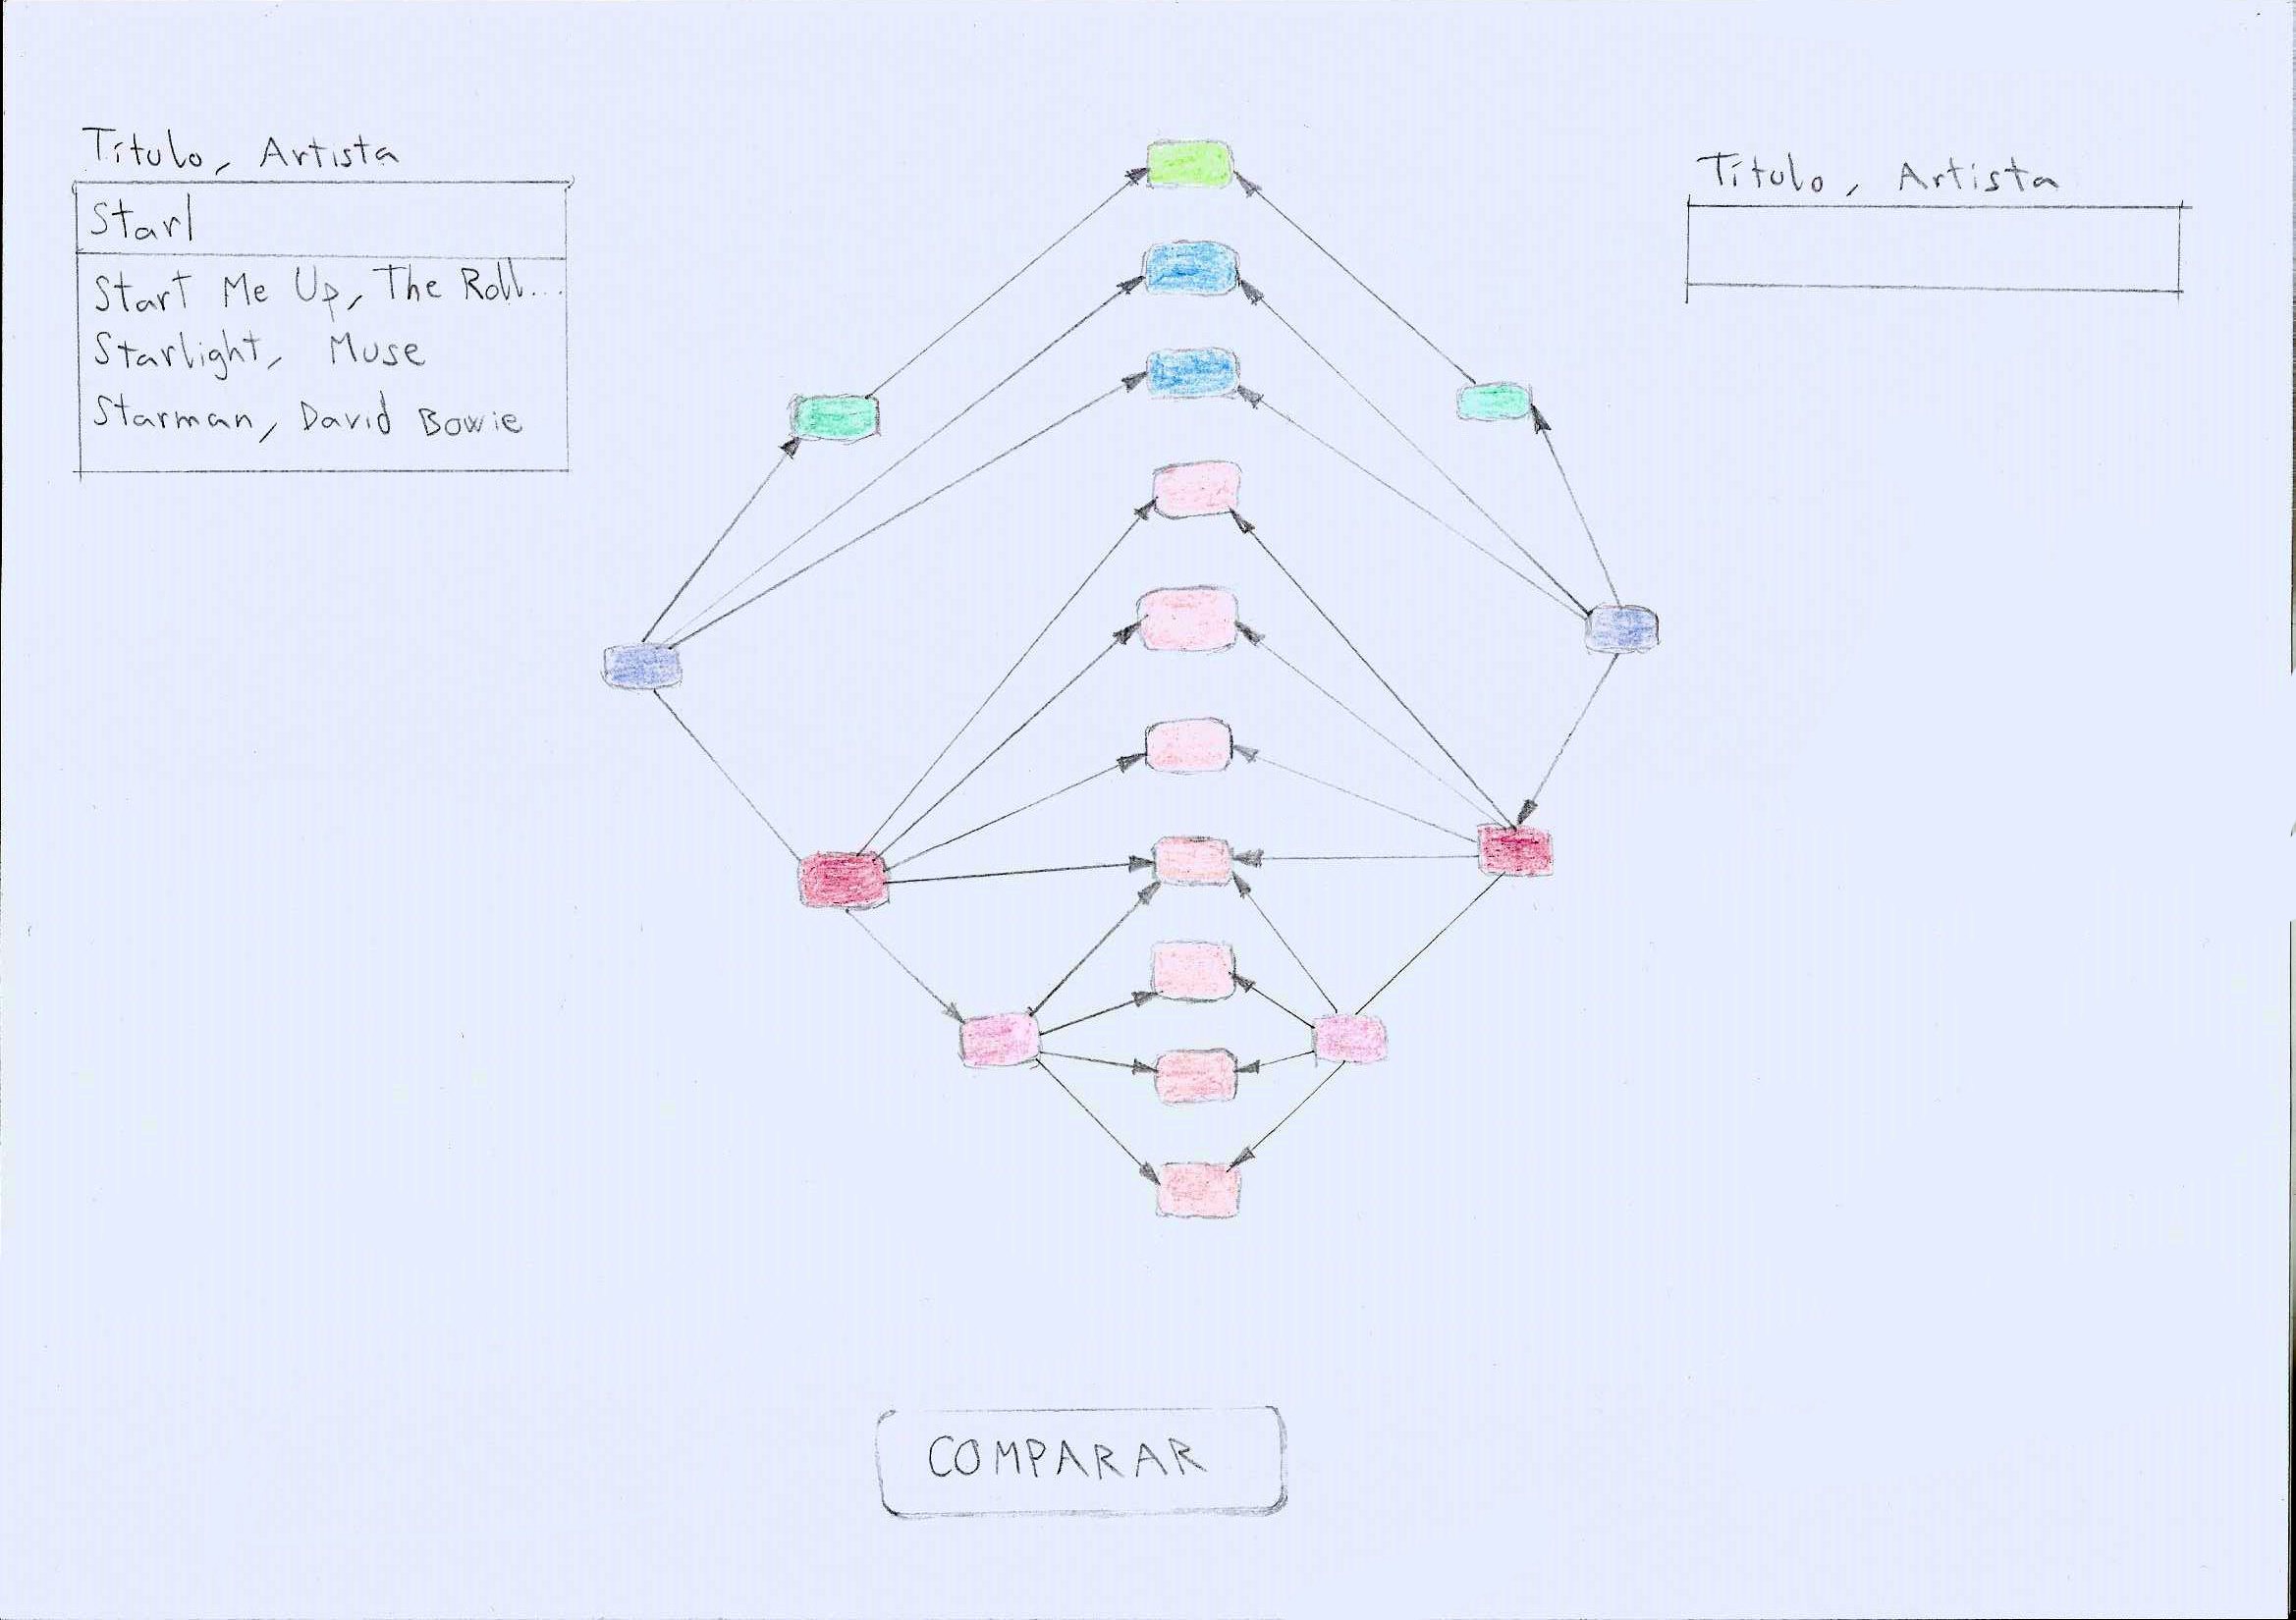
\includegraphics[width = 0.9\textwidth]{Imagenes/Bitmap/Segunda Interfaz.jpg}
	\caption{Segundo diseño de la interfaz web}
	\label{fig:sampleImage}
\end{figure}

El resto de la interfaz consiste en los elementos con los que interactuará el usuario antes de generar el grafo de explicaciones. A ambos lados de la pantalla se sitúan los campos a rellenar con los datos básicos de las canciones. Para identificar la canción deseada es necesario escribir en ellos el título de la canción y el nombre de su artista, separados por una coma. En realidad este campo de entrada es un buscador que mostrará en un desplegable la lista de canciones que coinciden con el texto introducido y el usuario deberá seleccionar la que está buscando. Si intenta comparar una canción no contemplada por el sistema, aparecerá un mensaje de error.\\

La decisión de limitar las posibles entradas ha sido tomada por motivos prácticos. En Wikidata hay una cantidad ingente de temas musicales registrados, sin embargo los datos de cada canción concreta no siempre son tan completos como cabría esperar. A menudo falta información o la que hay no aparece siguiendo los mismos estándares que el resto, especialmente cuando se trata de canciones menos populares. Por ello hemos elaborado una lista de canciones que poseen información útil en Wikidata y que podemos tratar en nuestra aplicación sin problemas.\\

Por último, en la parte inferior de la pantalla hay un botón para ``COMPARAR’’. Una vez rellenados los campos de las dos canciones con opciones válidas, el usuario deberá pulsar este botón para que se dibuje el grafo de explicaciones. La primera vez que se use la aplicación no aparecerá ningún grafo en el centro de la interfaz, pero en las comparaciones siguientes el grafo previo no se borrará hasta pulsar de nuevo este botón para dibujar un grafo nuevo.\\

\section{Diseño avanzado}

\begin{figure}[h!]
	\centering
	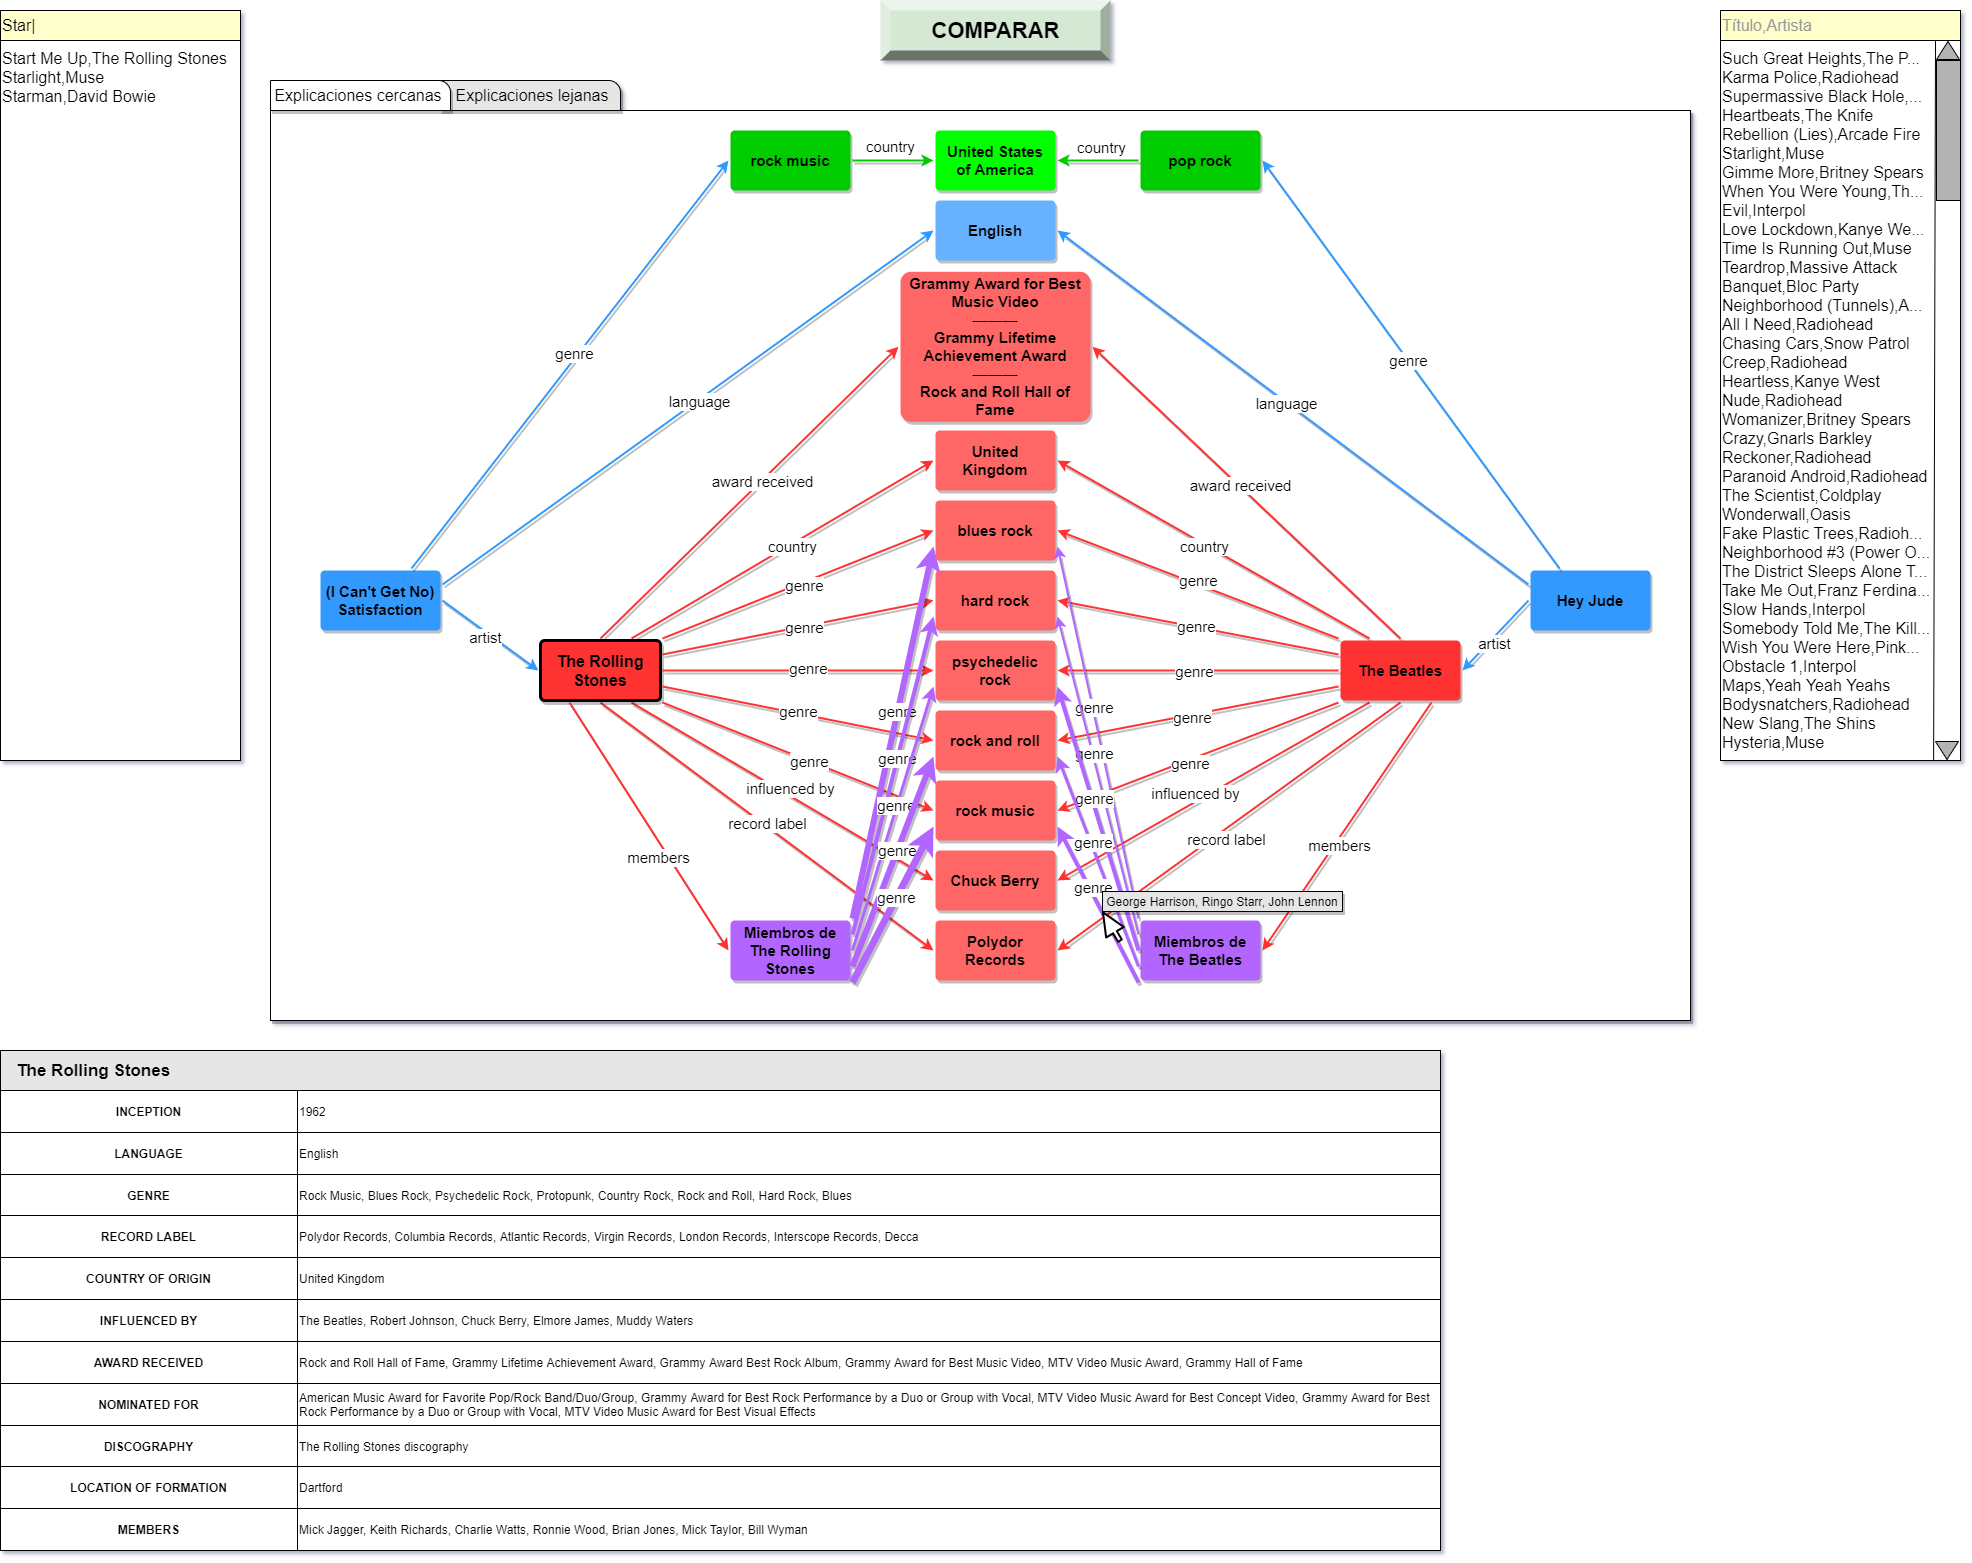
\includegraphics[width = 1\textwidth]{Imagenes/Bitmap/Tercera Interfaz.png}
	\caption{Tercer diseño de la interfaz web}
	\label{fig:sampleImage}
\end{figure}

Partiendo de la base establecida en los apartados anteriores, hicimos un diseño más completo de la interfaz para nuestra aplicación. Aquí se puede ver el regreso de la sección inferior con datos adicionales de los artistas y las canciones, esta vez en forma de tabla para que sea más legible para el usuario.\\

También por motivos de visibilidad y comprensibilidad se ha desplazado el botón ``COMPARAR'' a la parte superior de la pantalla, además de mostrar una lista con todas las canciones disponibles bajo los campos de entrada. Esta decisión se ha tomado para tratar de evitar que el usuario se sienta perdido por la falta de opciones visibles al abrir la aplicación por primera vez. Cabe destacar que esta lista se sigue filtrando en función de la entrada que esté escribiendo el usuario, mostrando así cuáles son sus opciones en todo momento.\\

En esta iteración se hacen algunos cambios al grafo de explicaciones. Para empezar, el nombre de las explicaciones (el predicado según RDF) se traslada a las aristas. También se han unido todos los nodos que tengan las mismas aristas conectándolos a los mismos nodos padres, pues resultaba innecesario repetir todas esas aristas y entorpecía la lectura del grafo. En el ejemplo mostrado se aprecia este cambio en los premios recibidos por los artistas, que ahora están recogidos en un solo nodo.\\

De la misma forma se colapsan los nodos de los miembros de los artistas, reduciéndolos a un solo nodo por artista. Para expresar cuántos integrantes se ven involucrados en cada explicación, el grosor de la arista que los une varía en función del número de miembros que participan en esa explicación concreta. Además, al colocar el ratón sobre esas aristas aparece una etiqueta donde figuran los nombres de esos miembros. Este cambio se propuso para reducir el número de nodos y aristas, pues en ciertos casos podía ser abrumador a la vista.\\

Por último, cabe destacar las pestañas que se ven justo encima del marco para el grafo. Para tratar de mejorar la legibilidad lo máximo posible decidimos hacer dos grafos diferentes, siendo el que vemos en la Figura 4.3 el de ``explicaciones cercanas''. Este grafo muestra solamente las explicaciones existentes entre elementos del mismo ``nivel de estudio''. Esto quiere decir que, por ejemplo, el género de una canción solo podrá relacionarse con un género de la otra canción, pues corresponden al mismo estudio o categoría. Por el contrario, no se verán relaciones existentes entre ese género y otro elemento, como una canción, artista o miembro.\\

\begin{figure}[h!]
	\centering
	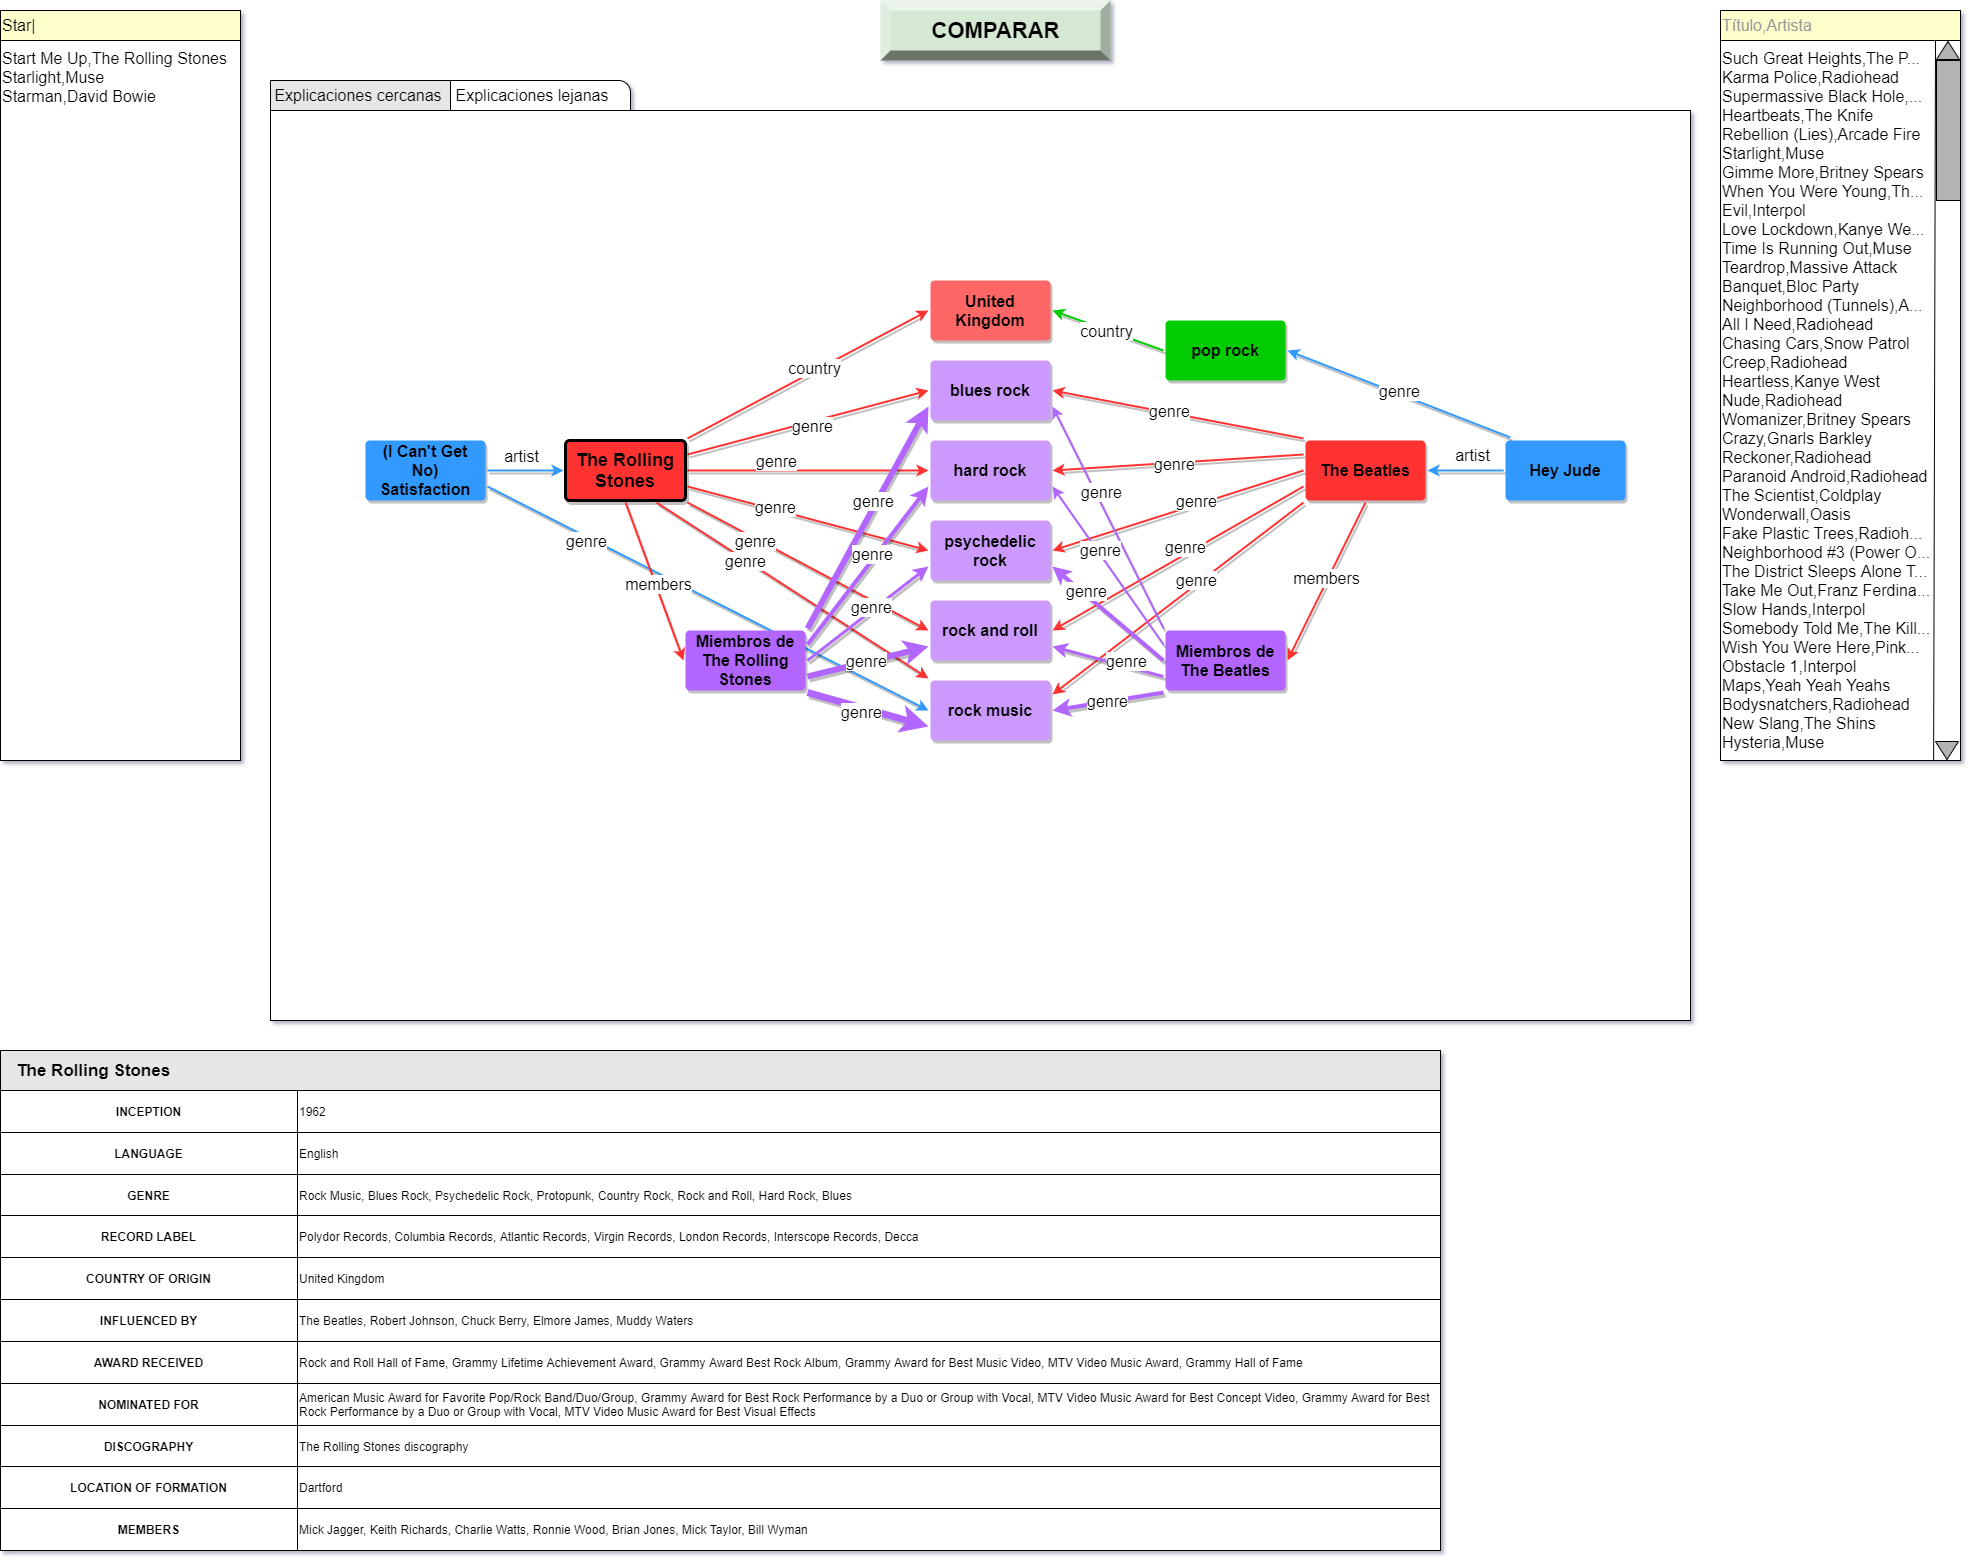
\includegraphics[width = 1\textwidth]{Imagenes/Bitmap/Tercera Interfaz (Alternativa).png}
	\caption{Grafo de explicaciones lejanas}
	\label{fig:sampleImage}
\end{figure}

En la Figura 4.4 se ve el llamado ``grafo de explicaciones lejanas'', con el que se ve mejor la diferencia. Al contrario del ``grafo de explicaciones cercanas'', aquí solo se muestran las explicaciones existentes entre elementos que pertenecen a estudios diferentes. De esta forma, en este grafo se ve la relación entre el artista \textbf{The Rolling Stones}, autor de la primera canción, y el género \textbf{pop rock} obtenido de la segunda canción.\\

El usuario podrá cambiar de vista libremente para consultar ambos grafos haciendo click en las pestañas anteriormente mencionadas. Todas las funciones explicadas en esta sección aparecen en ambos grafos.\\